\documentclass[12pt]{article}

% The geometry package al	lows for easy page formatting.
%\usepackage{geometry}
%\geometry{letterpaper}

% Load up special logo commands.
\usepackage{doc}
\usepackage{fullpage}
\usepackage{booktabs}
\usepackage{subcaption}
\usepackage{lmodern}

% Package for formatting URLs.
\usepackage{url}

% Packages and definitions for graphics files.
\usepackage{graphicx}
\usepackage{epstopdf}
\usepackage{natbib}
\usepackage{tikz}
\DeclareGraphicsRule{.tif}{png}{.png}{`convert #1 `dirname #1`/`basename #1 .tif`.png}

%
% Set the title, author, and date.
%
\title{Panthera: Caching and Cache-based
Scheduling in Distributed Computing Systems}
\author{Dhaivat Pandya \\ Appleton North High School}
\date{}
%
% The document proper.
%
\begin{document}

% Add the title section.
\maketitle

% Add an abstract.
\abstract{
	The adoption of distributed computing systems has grown massively in the past few years. In particular, Apache Hadoop, which allows developers to create applications that run on a cluster of computers, is currently used throughout academia and industry in areas such as machine learning, medical diagnosis, natural language processing, etc. However, the Hadoop File System fails to effectively utilize random access memory (RAM) and local storage in order to reduce waiting time (i.e. latency). In this project, named \textit{Panthera}, caching and scheduling systems for Hadoop were developed. \textit{Panthera} caches both information about files and the file contents, thereby reducing waiting time in downloading and accessing the files and related information. It runs with an unmodified version of Hadoop, meaning it can integrate easily into existing architecture. The results showed that data access latency was 8.63 times lower with \textit{Panthera} and metadata access latency was 8.13 times lower. Such drastic decreases in latency can greatly increase the efficiency of existing Hadoop applications and also allow the creation of algorithms that were previously not feasible on Hadoop. \textit{Panthera} was tested with existing Hadoop algorithms and running times were up to 3.31 times lower than the control group of a standard Hadoop installation. In addition to the caching system, a scheduler and scheduling algorithm for Hadoop were developed. They use information available about the caches to decide the order of execution for computational jobs, thereby further reducing running time. Finally, \textit{Panthera} is widely applicable and can significantly speed up research in a very large range of fields ranging from bioinformatics to artificial intelligence. All code developed during this project will be open sourced to further development in the area.
}

\section{Introduction}
As computational problems and their associated datasets have grown in size, it has become necessary to take advantage of distributed computing systems to solve them \cite{taylor2010overview}. Such systems allow programs to scale from one computer (i.e. one \textit{node}) to thousands of computers with few or no changes in the codebase. In particular, the Hadoop distributed system \cite{hadoop} has seen tremendous growth. Hadoop is an open source implementation of the revolutionary MapReduce system developed at Google \cite{mapreduce}. With it, developers can easily take advantage of large, multi-node clusters to solve computational problems.

Hadoop consists of a computational layer termed \textit{MapReduce} and a custom distributed filesystem named \textit{Hadoop Distributed File System (HDFS)}. HDFS is used to allow all nodes in a cluster access to the same dataset. For instance, one may consider running an algorithm that counts the frequency of each word in a large text file. If this algorithm is run on a Hadoop cluster, each node must have access to the file in question in order to determine word frequency.

Current Hadoop deployments exist in the thousands of nodes at companies such as Cloudera, Facebook, Yahoo, etc. Especially in such large networks, \textit{access latency}, or the waiting time associated with accessing files and related information through the Hadoop Distributed File System (\textit{HDFS}), is a significant concern \cite{hdfs}. Latency in distributed systems can have significant effects and a reduction of the same comes with tremendous benefits. As the RAMCloud project has outlined \cite{ramcloud}, low latency can greatly extend the applications of distributed computing systems. For example, algorithms that require files other than the input file are largely impractical in high latency systems such as Hadoop \cite{ramcloud, spark}. A similar case exists with jobs (or sets of jobs) that consist of multiple passes over the same dataset; many of these exist in the field of machine learning, analytics, etc. \cite{spark}. However, with lowered latency, such algorithms may become useful and applicable. HDFS currently does not use local (i.e. on the client) random access memory (RAM) to improve latency.

I present \textit{Panthera}, a \textit{cache layer} and \textit{cache-based scheduling system} for Hadoop. The \textit{Panthera} cache layer functions by retaining recently accessed files and related information in random access memory. Thus, when the files are needed once again, they do not have to be downloaded or read from the hard drive, thereby greatly reducing file access latency. Another portion of the project, the \textit{Panthera} scheduling system utilizes information about the data blocks cached in a cluster at a given time to schedule jobs. By doing so, it aims to maximize the benefit of caching to a series of jobs.

In this paper, the \textit{Panthera} caching layer and scheduling system are presented. In Section \ref{sect:architecture}, motivation and construction of the \textit{Panthera} architecture are explained. Section~\ref{sect:caching_layer} describes the caching layer portion of this project. Section~\ref{sect:scheduler} presents the scheduling algorithm and implementation details. The results and data are noted in Section~\ref{sect:results}. Finally, Sections \ref{sect:conclusions}, \ref{sect:applications}, \ref{sect:future_work} conclude with an interpretation of the results, discussion of potential applications and future work.

\section{Architecture} \label{sect:architecture}
\subsection{Design Constraints}  \label{design_constraints}
The primary goal of the \textit{Panthera} project is to reduce access latency in HDFS. Therefore, data and metadata request latency should be significantly lowered with \textit{Panthera} in comparison to the control group of a standard Hadoop installation. 

There are many systems built on Hadoop that are in widespread use \cite{hbase, cloudbatch, pig}. The Hadoop project is also supported by large corporations with a 
consistent release cycle. Thus, for \textit{Panthera} to be practical, it must opedrate independently of the existing Hadoop codebase, i.e. as a layer, rather than modification. This implies that \textit{Panthera} must implemented without a single change in the existing Hadoop codebase, i.e. as a ``drop-in'' solution. This is due to the fact that a deviation from the mainline Hadoop codebase would have to updated at the same pace as the vanilla Hadoop, which would be contrary the benefits of Hadoop's large and active development community.  Also, since \textit{Panthera} does not require any code modifications to existing Hadoop applications, allowing it to be easily integrated into current software stacks. 

In order to develop a cache-based scheduling system, the \textit{Panthera} caching layer must be able to report information (e.g. blocks currently cached) over the network. The cache-based scheduler then uses information about blocks cached and the files each job requires to run in order to optimize the running order of a set of jobs (see Section \ref{sect:scheduling} for a complete description of the \textit{Panthera} scheduling algorithm).

\subsection{Metadata and Data} \label{metadata_and_data}

Within the Hadoop File System (HDFS), there is a clear architectural distinction between \textit{metadata} and \textit{data} \cite{hdfs}. Metadata refers to information about a file or a directory, e.g. file size, file names, the location of a file in the cluster, etc. For HDFS, the NameNode server handles all metadata. For every request, the NameNode recomputes metadata. \textit{Panthera} can reduce this computation by caching the results of a previous request, thereby conserving resources.

Data refers to the actual content of a file. Within HDFS, each file is split into 64 MB large \textit{blocks}, which are stored on DataNodes. Here, \textit{Panthera} serves to reduce access time by holding recently used blocks in RAM locally thereby eliminating the need to download files from a remote server if they are present in the cache.

Metadata and data caching provide significantly different technical challenges as the former involves conversion of computational latency to memory latency, whereas the latter involves a conversion of network and hard drive latency to memory latency. Note: memory latency is of the smallest magnitude of all three in consideration. In many cases \cite{ramcloud} it is 1/1000th hard drive latency.

\subsection{Panthera Architecture} \label{architecture_sect}
\begin{figure}
\centering
\begin{subfigure}{.5\textwidth}
  \centering
  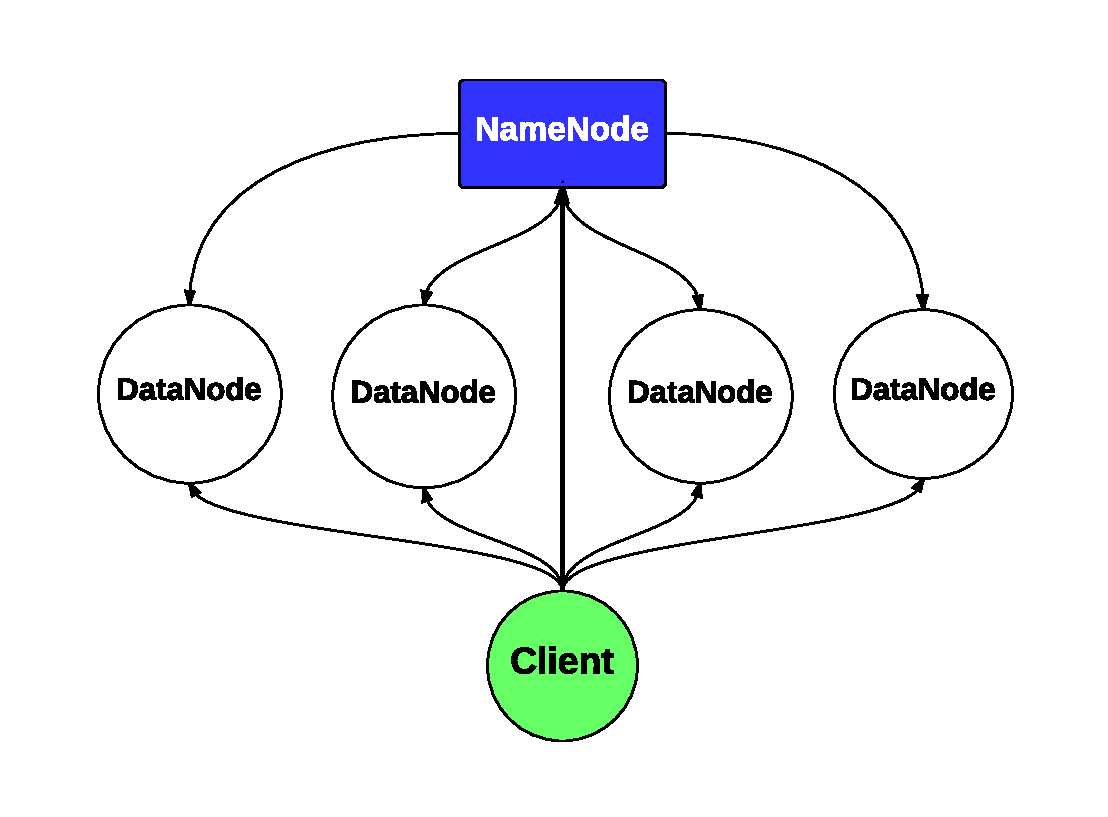
\includegraphics[scale=0.4]{assets/hadoop_architecture.pdf}
  \caption{Vanilla Hadoop architecture}
  \label{fig:vanilla_arch}
\end{subfigure}%
\begin{subfigure}{.5\textwidth}
  \centering
  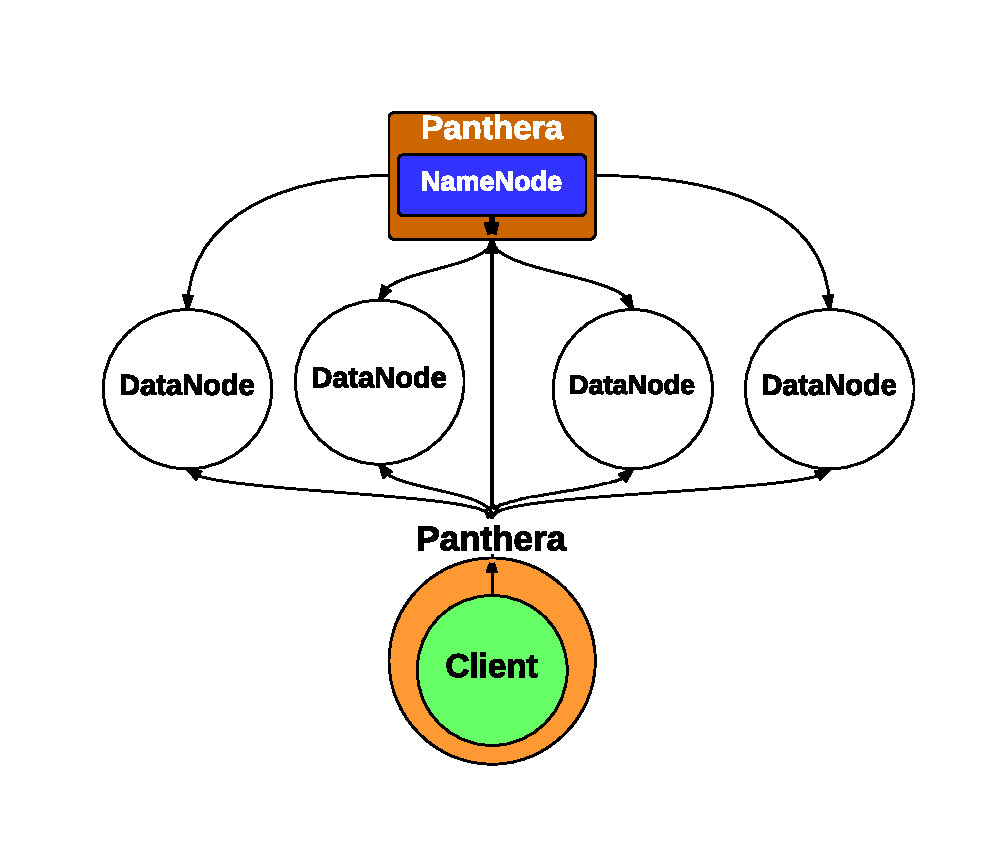
\includegraphics[scale=0.4]{assets/panthera_architecture.pdf}
  \caption{Panthera-Hadoop architecture}
  \label{fig:panthera_arch}
\end{subfigure}
\label{fig:arch}
\end{figure}


Figure~\ref{architecture_sect} outlines the architecture differences between a standard Hadoop File System architecture and an installation with \textit{Panthera}. In HDFS, the \textit{NameNode} serves as a metadata server, handling all requests from clients relating to metadata (e.g. directory listing, file sizes, block locations, etc.). \textit{DataNode(s)} hold data and serve it at request from the client. In order to read or write a file, a client first obtains permission from the NameNode and subsequently communicates with a DataNode to complete the operation. Though the aforementioned background is sufficient for this paper, a more complete description of the Hadoop File System may be found in \cite{hadoop}.

\textit{Panthera} operates by intercepting requests and responses at the NameNode and the client. Both nodes have a running instance of \textit{Panthera}. Every request issued from the client is first reviewed by \textit{Panthera}, and if possible, answered immediately from the cache. If the response is not found in the cache, certain requests are cached and subsequent responses are associated with the request in consideration.

The \textit{Panthera} instance on the NameNode serves as a cache refresh mechanism. Though sparse in the Hadoop environment since input files are usually not written to in the MapReduce computational paradigm, files that are cached may become out-of-date, i.e. the cache becomes "stale". The \textit{Panthera} instance on the NameNode monitors the filesystem for changes and reports certain changes to Panthera caches, which then remove stale files from the cache. The refresh mechanism is particularly important for metadata caching where the cached information is far more likely to change during the execution of a job.

The \textit{Panthera} cache layer, since it caches both data and metadata, can be considered two separate subsystems, which are now discussed.

\section{Panthera Caching Layer} \label{sect:caching_layer}
A significant portion of Panthera is a caching layer for Hadoop, the details of which are now covered. 
\subsection{Metadata caching} \label{sect:metadata_caching}

\begin{figure}[!h]
	\caption{\textit{Panthera} Metadata System}
	\centering
		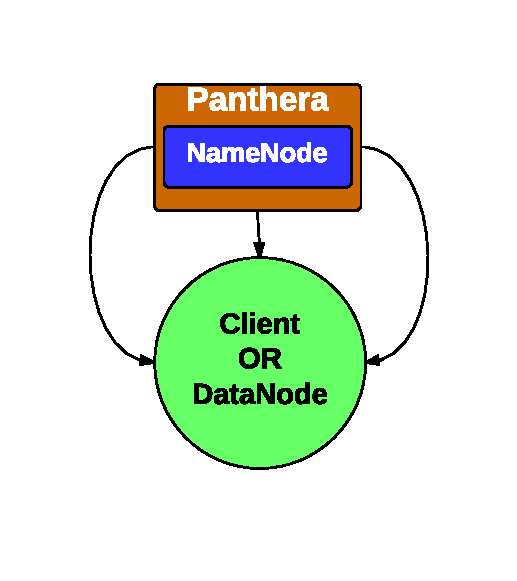
\includegraphics[scale=0.4]{assets/panthera_meta_architecture.pdf}
\end{figure}

The \textit{Panthera} metadata system runs on the NameNode and communicates with the \textit{Panthera} instance on the client. The challenge on the metadata portion consists of converting computational latency to memory latency. For example, for some intensive methods (e.g. a recursive directory listing), it may be worthwhile to cache a response in order to prevent computing the same list again.

However, the problem lies in identifying such methods. Obviously, there are some methods for which caching is not worthwhile since their execution time is lower or comparable to memory latency. Within Hadoop, there are several methods that incur very significant computational latency, e.g. a recursive directory listing. Only these methods are cached within Panthera.

Currently, a standard LRU cache \cite{cache} is used for each method. Testing of different caching methods and predictive prefetching algorithms \cite{griffioen} is under way.

\subsection{Data caching} \label{sect:data_caching}

\begin{figure}[!h]
	\caption{\textit{Panthera} Data System}
	\centering
		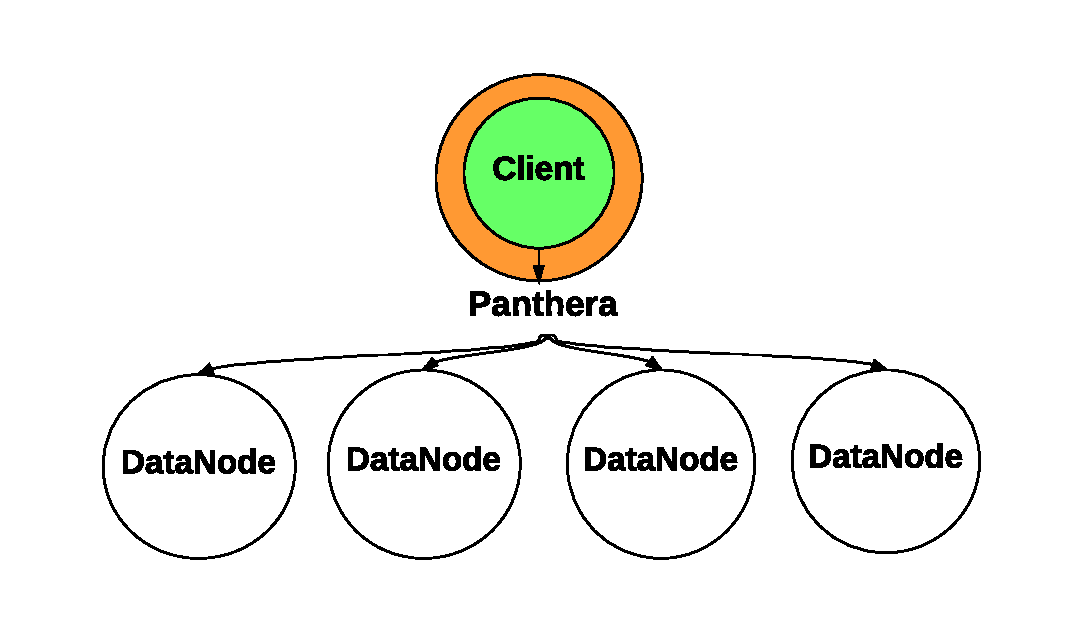
\includegraphics[scale=0.4]{assets/panthera_data_architecture.pdf}
\end{figure}

\textit{Panthera}'s data caching system runs on the client. The architecture is similar to that of the metadata caching system. Every request that the client makes to the DataNodes is first processed by \textit{Panthera} and responded to from the cache if possible. 

The challenges with data caching differ significantly from those in metadata caching. Here, the goal is to convert network and hard drive read latency into memory latency. As \cite{ramcloud, hadoop} note, memory latency can be extremely low in modern systems, especially in comparison to network and hard drive latencies. Thus, in some respects, the goal of lowered latency is ``easier'' to attain in the data cache in comparison to the metadata cache. 

\section{Scheduler} \label{sect:scheduler}
\subsection{Hadoop Job Structure}
Hadoop, in professional and academic environments, is often used with series rather than individual jobs. For example, in machine learning, various algorithms (termed \textit{iterative machine learning algorithms}) consist of multiple Hadoop jobs rather than a single job \cite{spark}. In Hadoop-based querying systems \cite{hive, pig}, a set of queries may consist of jobs that are entirely independent of one-another. Deciding how to order these jobs depending on cached file availability is a problem of great interest; \textit{Panthera} presents the solution of a cache-based scheduler for Hadoop.

\subsection{Cluster Saturation}
It may be asked why it is not possible to run independent jobs in parallel on the Hadoop cluster. Each node in a given cluster has a maximum number of \textit{map} or \textit{reduce} calls (i.e. the basic computational units in Hadoop) it may process at a given time. If a job saturates nodes in a cluster, running another job concurrently would provide no running time benefit. Thus, a scheduler is useful since it may organize independent jobs in a beneficial ordering. In \textit{Panthera}, this ordering is based on the files or blocks present in the cluster's caches.

\subsection{Scheduling Algorithm} \label{sect:scheduling}

The scheduling problem faced may be stated as: 

\begin{quote}
Given $\mathbf{J} = J_1, J_2, ... ,J_k$ jobs to be run on a Hadoop cluster with caches $\mathbf{C} = C_1, C_2, ..., C_n$, what ordering will best take advantage of the caches?
\end{quote}

Each $J_i$ accesses a set of blocks $F_i$ and each $C_i$ holds a set of blocks $B_i$. \textit{Panthera} assigns every $J_i$ a \textit{job score}, denoted $x_i$:
			\begin{equation}
				x_i = \displaystyle{\frac{\left\vert{F_i \cap B_t}\right\vert}{ \left\vert{B_t}\right\vert}} \; \textrm{where} \;
				B_t = \bigcup_{j = 1}^{n} B_j
			\end{equation}
			
			The \textit{Panthera scheduling algorithm} consists of sorting $\mathbf{J}$ in descending order with respect to the $x_i$ associated
			with each $J_i$. 
			
		While $J_i$ is running, \textit{Panthera} may prefetch data for $J_{i+1}$ to further reduce latency. An implementation of predictive prefetching algorithms as described in \cite{griffioen1994reducing} is possible in \textit{Panthera} and may serve to further reduce latency in specific applications.

\section{Results} \label{sect:results}

\subsection{Testing Methodology}
In order to test the metadata cache, a directory listing query was repeatedly run on a directory with 100 files in it, and the latency times for responding are measured, with \textit{Panthera} and without. The reasoning for picking such a test lies in the fact that a directory listing in Hadoop involves all six of the cached methods as well as a few non-cached methods. Thus, the test provides a good estimate of the efficacy of the cache. Latency times for the data cache were obtained by repeatedly querying for a 64 megabyte large file. The file size was chosen since it is the default block size for a Hadoop cluster and the \textit{Panthera} cache stores files as blocks. Both metadata and data cache testing was conducted on virtualized server instances running on hardware with solid state hard drives. 

In order to test the effects of \textit{Panthera} on the Hadoop computing system (rather than focusing on only HDFS access time), running times of two existing algorithms were recorded. The first is \textit{WordCount}, the classic distributed algorithm that counts the number of occurrences of each word in a text file. The second has been, termed \textit{RefCount}, has thus far been impractical on Hadoop due to excessive running times. It is similar to WordCount in that it counts occurrences of words, but it consults a \textit{reference file} (e.g. a limited dictionary) to determine which words are to be counted.

\subsection{Results}
\begin{figure}
\centering
\begin{subfigure}{.5\textwidth}
  \centering
  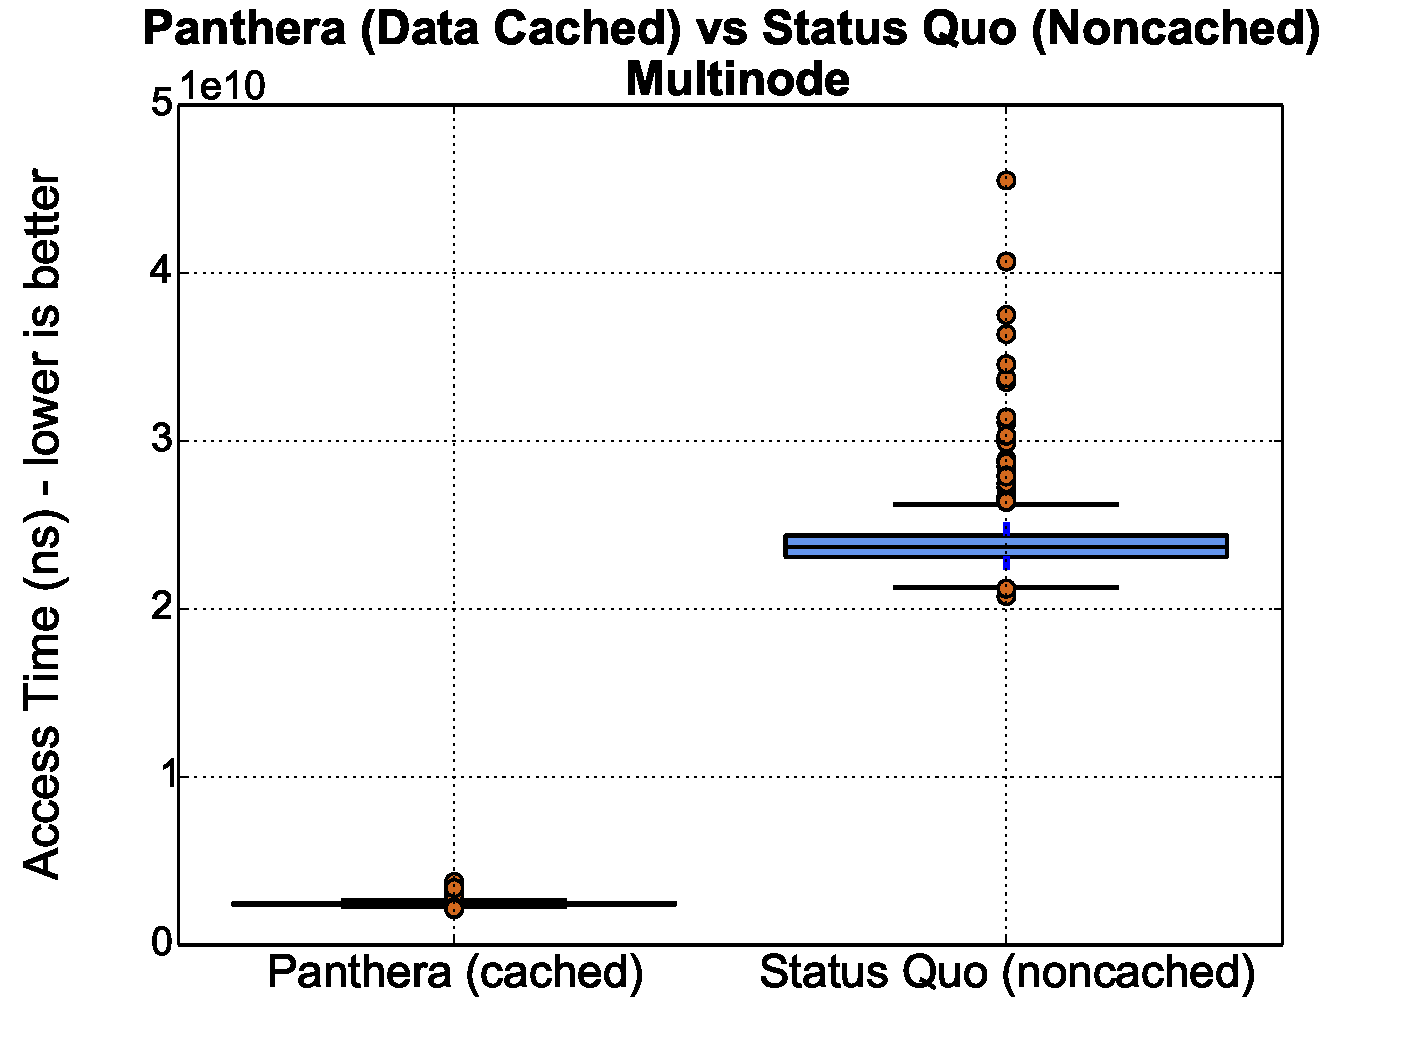
\includegraphics[scale=0.3]{assets/v2/getter_boxplot.pdf}
  \caption{Data access latency}
  \label{data}
\end{subfigure}%
\begin{subfigure}{.5\textwidth}
  \centering
  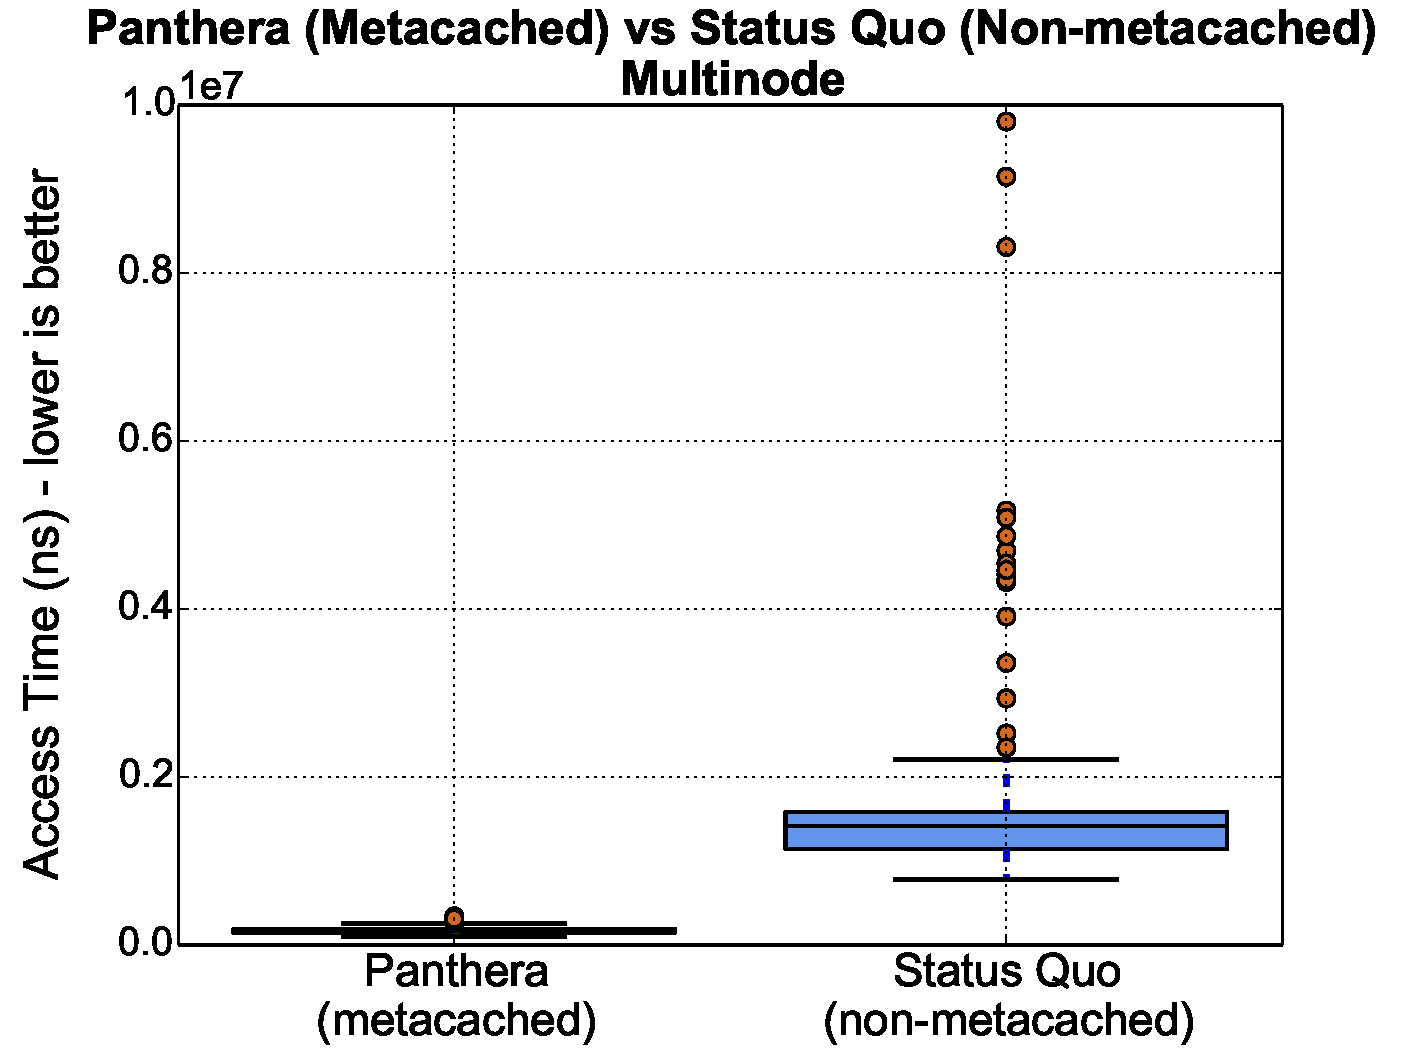
\includegraphics[scale=0.3]{assets/v2/multinode_meta_box_plot.pdf}
  \caption{RefCount job performance}
  \label{meta}
\end{subfigure}
\caption{Metadata access latency}
\label{fig:test}
\end{figure}


	\begin{table}
	\centering
			\begin{tabular}{lcc}
			\toprule
			\textbf{Type} & \textbf{Mean Time Improvement} & \textbf{Standard Dev. Contraction} \\
			\midrule
			Metadata   & 8.13x & 27.38x \\
			Data       & 8.63x & 11.14x \\
			WordCount & 1.25x & \phantom01.02x \\
			Ref. count & 3.31x & 22.91x \\
			\bottomrule
			\end{tabular}
		\caption{Latency improvement with \textit{Panthera}}
		\label{results}
	\end{table}

	
The \textit{Panthera} data cache decreased file access latency by a factor of 8.63 and metadata access latency was lowered by a factor of 8.13, both representing drastic decreases in HDFS latency. In addition, the standard deviation was also significantly decreased with \textit{Panthera}: by a factor 27.38 for metadata and a factor of 11.14 for data. With a lower standard deviation, the predictability of performance for Hadoop applications increases.

The tests with existing Hadoop algorithms show similarly positive results. \textit{Panthera} is able to reduce running time for the WordCount algorithm by 25\% and is able to do the same for the Ref. Count algorithm by 331\%. It is important to keep in mind that these performance boosts were attained with the original algorithms left entirely unmodified. The difference between the two lies in the fact that WordCount has little interaction with HDFS once the initial input files have been downloaded, whereas Ref. Count often obtains the reference file from HDFS. Notice that the testing was conducted with only one slave node. Adding slave nodes to a cluster would increase the number of file requests since each node requires a portion of the input file. 

\begin{figure}
\centering
\begin{subfigure}{.5\textwidth}
  \centering
  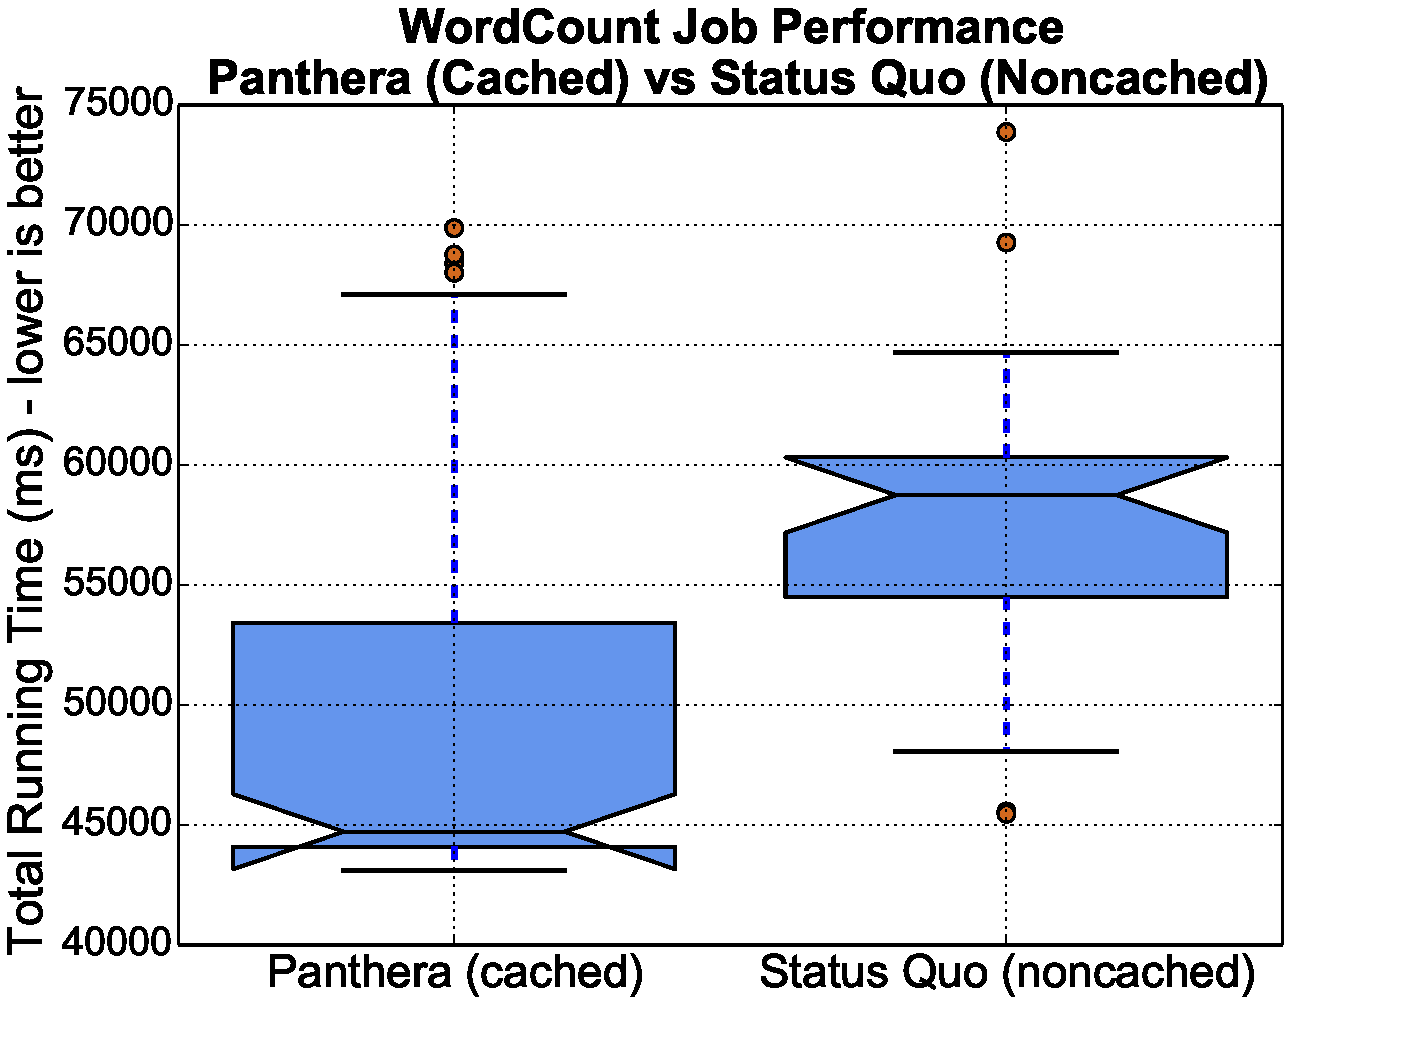
\includegraphics[scale=0.3]{assets/v2/wordcount_boxplot.pdf}
  \caption{WordCount job performance}
  \label{fig:sub1}
\end{subfigure}%
\begin{subfigure}{.5\textwidth}
  \centering
  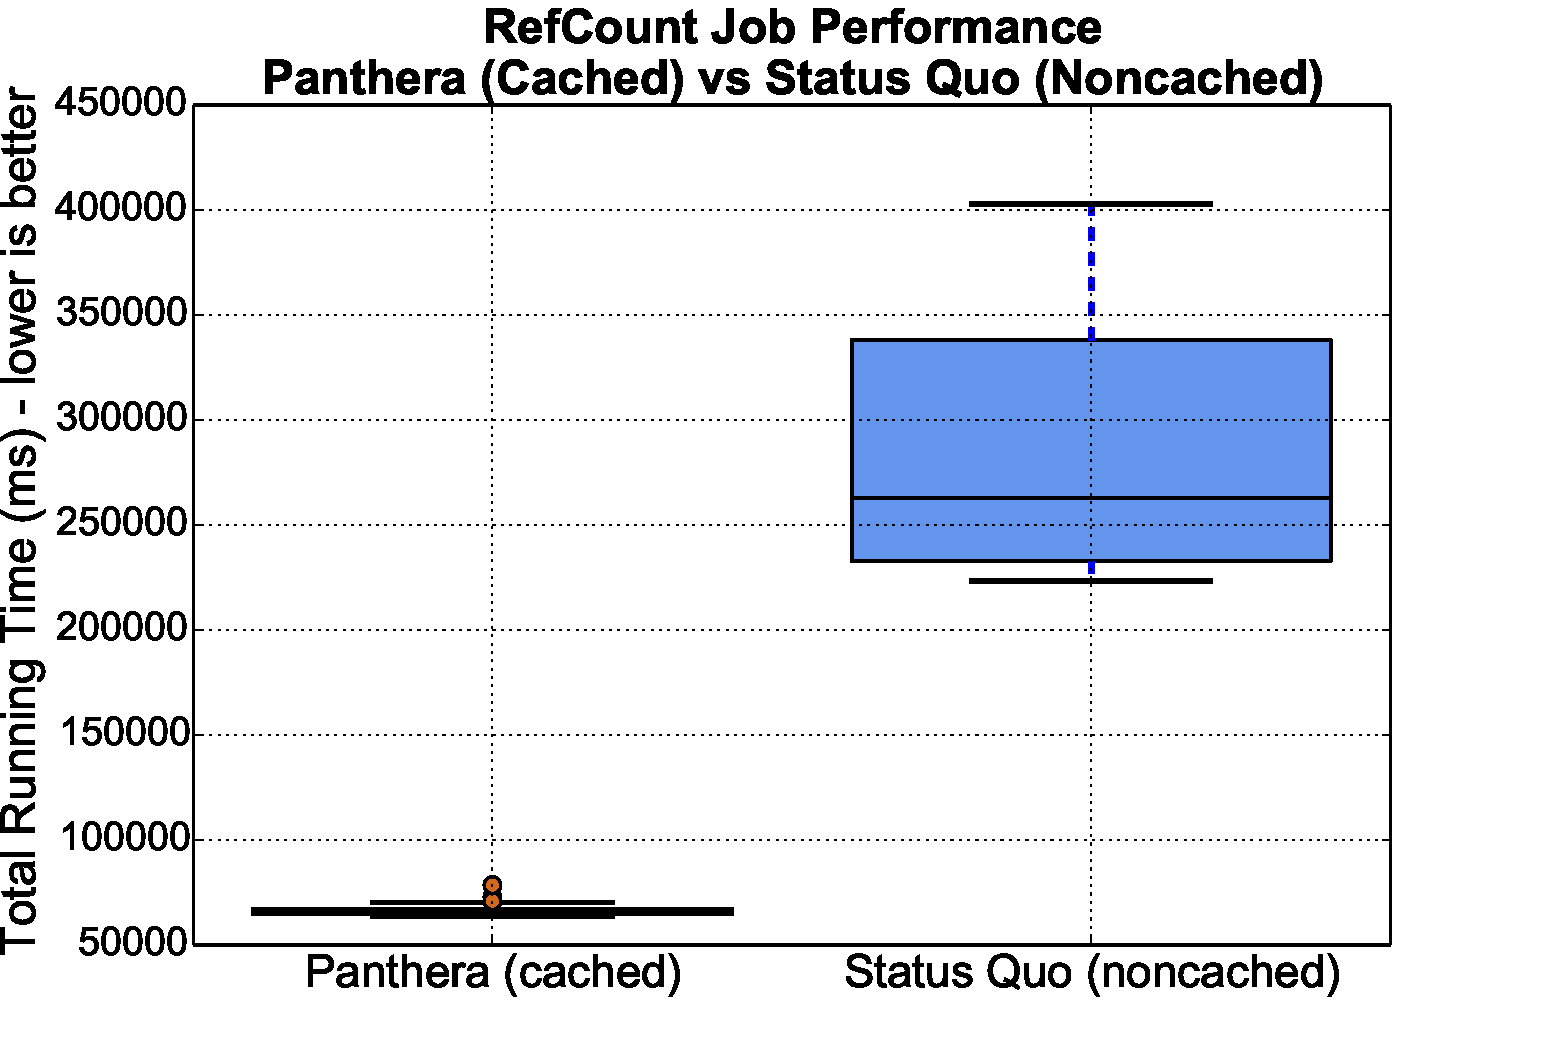
\includegraphics[scale=0.3]{assets/v2/refgetter_boxplot.pdf}
  \caption{RefCount job performance}
  \label{refgetter}
\end{subfigure}
\caption{Algorithm running time comparison}
\label{fig:test}
\end{figure}

\section{Conclusions}\label{sect:conclusions}

\textit{Panthera} fulfils all of the constraints mentioned at the outset. It is a layer on Hadoop rather than a main repository code modification, allowing existing Hadoop applications to remain entirely unmodified. Considering the latency measurements, it is clear that it has also met the requirements in terms of benefit. \textit{Panthera} was able to reduce data access latency by a factor of 8.63 and reduce basic metadata access latency by 8.13. Also, \textit{Panthera} was able to minimize the spread of latency times in both data and metadata requests. Thus, \textit{Panthera} opens up great possibilities within Hadoop due to the fact that algorithms that were previously impractical (e.g. distributed tree traversal algorithms) may now be implemented. Additionally, a scheduler algorithm was devised and a cache-based scheduler was implemented for Hadoop which enables further reduction of latency via greater utilization of cached resources.

Previous work \cite{hdfs, borthakur2011apache} has lamented the latency issues that have plagued HDFS and Hadoop as barriers to adoption. \textit{Panthera} significantly reduces the scope of these issues and allows the application of Hadoop in areas where its reach has been limited.

\section{Applications}\label{sect:applications}
One of the major benefits of the systems developed is that they are independent of the existing Hadoop codebase and they do not require modifications to existing Hadoop applications. Thus, \textit{Panthera} may be deployed in a wide range of scenarios, such as the following:

\begin{itemize}
	\item Bioinformatics: Hadoop is currently in use in bioinformatics research \cite{taylor2010overview}. Panthera can be employed to reduce access latencies of various datasets, e.g. protein data banks, etc. Additionally, domain-specific prefetching can be performed to further improve performance.
	
	\item Machine learning: Apache Mahout is a machine learning library for Hadoop. Panthera has been tested with the K-Means implementation it provides and there is evidence of significant performance improvement.
	
	\item Predictive analytics: A quickly growing field that has thoroughly
	embraced Hadoop \cite{chen2012business}. Metadata caching can be used to decrease human operator waiting time. Often, queries consist of several queued jobs, meaning that the \textit{Panthera} scheduler can be used to optimize
	job ordering.
\end{itemize}

\section{Future work}\label{sect:future_work}
One of the most immediate avenues for further research is in \textit{domain-specific prefetching}. Different problem domains (e.g. natural language processing, predictive analytics, etc.) have different dataset requirements. It may be possible to predict what files a given job will need depending
on what problem domain the job is in. A generalized version of the same problem would be \textit{predictive prefetching} \cite{griffioen1994reducing} which involves the prediction and prefetching of files that will be required in the future. In both these problems, the Hadoop environment provides unique
challenges.


Another area worthy of further exploration is the effect of different cache replacement algorithms in Hadoop. Though various cache replacement algorithms
have been explored thoroughly at the local filesystem level, their study 
in conjunction with existing Hadoop algorithms may provide novel results, i.e.
the access patterns of certain procedures may work best with a certain
cache replacement scheme \cite{puzak1985analysis}.

\nocite{*}

\bibliographystyle{plain}
\bibliography{references}

\end{document}